\documentclass{article} % For LaTeX2e
\usepackage{nips15submit_e,times}
\usepackage{hyperref}
\usepackage{url}
%\documentstyle[nips14submit_09,times,art10]{article} % For LaTeX 2.09
\usepackage[pdftex]{graphicx}  % omogoča vlaganje slik različnih 
\usepackage{wrapfig}
\usepackage{caption}
\usepackage{subcaption}
\usepackage{listings}
\usepackage{natbib}
\usepackage{todo}
\newtheorem{theorem}{Theorem}[section]
\usepackage{amsmath}
\usepackage[]{algorithm2e}






\title{Neural network pruning with simultaneous matrix tri-factorization}
\author{Teja Ro\v{s}tan}
%\template is for anonymous submission

% The \author macro works with any number of authors. There are two commands
% used to separate the names and addresses of multiple authors: \And and \AND.
%
% Using \And between authors leaves it to \LaTeX{} to determine where to break
% the lines. Using \AND forces a linebreak at that point. So, if \LaTeX{}
% puts 3 of 4 authors names on the first line, and the last on the second
% line, try using \AND instead of \And before the third author name.

\newcommand{\fix}{\marginpar{FIX}}
\newcommand{\new}{\marginpar{NEW}}

\nipsfinalcopy % Uncomment for camera-ready version

\begin{document}


\maketitle

\begin{abstract}

In this paper we present an approach for pruning neural networks, which
significantly reduces the model size and running time while maintaining its 
generalization performance. We apply a simultaneous matrix tri-factorization 
to map weight matrices to a low-dimensional space, therefore reducing them 
and partially eliminating noise. Factorized models are thus more robust and 
have a better generalization ability.

\end{abstract}

\section{Introduction}

Deep neural networks are a popular tool that is being used to solve widely
different problems. They are widely used for complex or abstract problems 
such as image,
sound and text recognition. However, they are computationally intensive to
train and are known for black box problem as they will not tell you why they
reached a certain conclusion. Success of neural networks largely depends on
their architecture. While the size of the input layer and the output layer is
known, the number of hidden layers and the number of nodes in each hidden layer
depends on the complexity of the problem~\cite{augasta2013pruning}. Generally,
a network with large number of hidden nodes is able to learn fast and avoids
local minima, but when a network is oversized, the network may overfit the
training data and lose its generalization ability while still having
unnecessary calculations as they are using more nodes than necessary. Better
generalization performance can be achieved only by small networks. They are
easier to interpret but their training may require a lot of effort. Also too
small networks are very sensitive to initial conditions and learning parameters
and do not generalize well. The most popular approach to
obtain the most optimal architecture of neural network is pruning. Pruning is
defined as a network trimming within the assumed initial architecture, which is
larger than necessary. Pruning algorithms are used to remove the redundant
connections while maintaining the networks performance. So one can use the
larger networks for training and its generalization can be improved by the
process of pruning~\cite{augasta2013pruning}.

More recent researches have tackled upon an issue of deep learning which is 
that they involve many layers with
millions of parameters, making the size of the network model to be extremely
large to store and with high computation cost. This prohibits the usage on 
resource limited hardware
especially mobile devices or other embedded devices even though deep neural
networks are increasingly used in applications suited for mobile
devices~\cite{DBLP:journals/corr/GongLYB14}.

In this work we present a novel approach using low-dimensional matrix
factorization. With pruning we wanted to acknowledge all relations that exists 
in network.
We used simultaneous matrix tri-factorization, also known as data fusion for 
dense layers and non-negative matrix factorization for convolutional layers. 
Pruning with these approaches was named matrix
factorization-based brain pruning (MFBP).


\section{Related work}

Because there is significant redundancy in the parametrization of networks,
many researchers found solutions to prune neural networks with possible
accuracy loss in order to reduce the model size extensively. But were able to
fine-tune the compressed layers with added learning iterations to recover the
performance and improve the accuracy back. In convolutional neural network, 
about 90\% 
of the model size is taken up by the dense connected layers and more than 90\% 
of the running time is taken by the convolutional 
layers~\cite{zeiler2014visualizing}. 

Compressing the most storage demanding dense connected layers is possible by
neural network pruning with low-rank matrix factorization
methods~\cite{bondarenko2014artificial, schmidhuber2015deep, sainath2013low},
where network pruning has been used both to reduce model size and to reduce
over-fitting~\cite{han2015learning}. State-of-the-art 
approaches~\cite{lecun1989optimal, hassibi1993optimal} opened a rich field of 
studies using matrix factorization to prune the networks.

Besides neural network pruning with matrix factorization many alternatives have
been used in numerous ways to optimize neural network architecture. One of the
latest studies~\cite{DBLP:journals/corr/GongLYB14} used vector quantization
methods for which they said have a clear gain over existing matrix
factorization methods. Alternative approach~\cite{xue2013restructuring} is
application of singular value decomposition (SVD) on the weight matrices to
decompose and reconstruct the model based on the sparseness of the
original matrices. A simple solution to
reduce the model size and preserve the generalization ability is to train
models that have a constant number of simpler neurons which was presented in
article~\cite{collins2014memory}. Another examined strong method uses the 
significance of neurons by evaluating
the information on weight variation and consequently prune the insignificant
nodes~\cite{han2015learning}. There the first phase learns which 
connections are important and removes the unimportant ones using multiple 
iterations. Hashing is also an effective strategy for dimensionality reduction
while preserving generalization performance~\cite{weinberger2009feature,
shi2009hash, chen2015compressing}. 

Running time complexity is depended from the computation which is dominated by 
convolution operations in the lower layers of the model. In contrast to model 
size compression, fewer approaches focused on reducing the time complexity. One 
of the earlier approaches of reducing the 
time complexity is FFT algorithm~\cite{mathieu2013fast} which by computing the 
Fourier transforms of the matrices in each set efficiently performs 
convolutions as pairwise products. However, the FFT based approach uses a 
significant
amount of temporary memory, since the filters must be padded to be the same size 
as the 
inputs~\cite{chetlur2014cudnn}. One approach is to lower the convolutions into a 
matrix multiplication 
by reshaping the filter tensor to provide performance as close as possible to 
matrix 
multiplication, while using no auxiliary memory~\cite{chetlur2014cudnn}. This 
avoids the usage of nested loops and speeds up the 
computation~\cite{chellapilla2006high}. 
However redundant data and kernels storage has its own cost 
of extra memory usage as said in article~\cite{anwar2015structured} where they 
also proposed to 
reduce this complexity with structured pruning and fixed point optimization. 

In articles~\cite{jaderberg2014speeding, rigamonti2013learning} they use an
intuition that CNN filter maps can be approximated using a low rank basis of
filters that are separable in the spatial domain where 
in~\cite{jaderberg2014speeding}
substantial speedups can be achieved by also exploiting the cross-channel 
redundancy to perform low-rank decomposition in the
channel dimension. 
Alternatively in article~\cite{denton2014exploiting} they compressed each 
convolutional layer by finding an appropriate low-rank approximation with 
considering several elementary tensor decompositions based on singular value 
decompositions, as well as filter clustering methods to take advantage of 
similarities between learned features.

Method, presented in article~\cite{zhang2015efficient}, takes the nonlinear 
units (ReLU) into account as they minimize the reconstruction error of the 
nonlinear responses, subject to a low-rank constraint which helped to reduce the 
complexity of filters, therefore reduced computation. 

\section{Approximation of weights in neural network}
\begin{figure}[!ht]
\centering
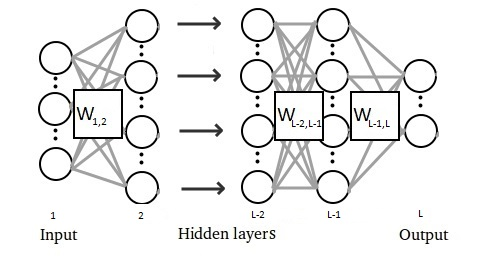
\includegraphics[width=.65\linewidth]{globokamreza2.jpg}
\captionof{figure}{Deep neural network with dense connected layers. Relation
matrix $W_{i,j}$ stores the weights of connections between neurons at layer $i$
and $j$.}
\label{f:globokamreza}
\end{figure}


Matrix factorization is a technique to search linear representation with
factorizing. Approximation of matrix with matrix factorization is used to
approximate the data in low-dimensional space in order to find latent features.

With ordinary artificial neural network, we have only one hidden layer and
therefore two weight matrices with sharing dimension. Because of this property,
we are able to concatenate the matrices through sharing dimension and apply a
matrix factorization. With deep neural networks~\ref{f:globokamreza} we have a 
multi-layer architecture where only
neighbour weight matrices share the same dimension. We can apply co-dependency
between neighbour weight matrices but we can not apply dependency between, for
example, first and third weight matrix. Our goal was to consider all relations
that exist between weight matrices in deep neural network. 

\subsection{Approximation of weights in dense layers}
Simultaneous matrix
tri-factorization applies our criteria for pruning in dense connected layers. 
The theorem of simultaneous matrix tri-factorization~\ref{t:2}. 


\begin{theorem}\label{t:2}
Simultaneous tri-factorization of multiple matrices simultaneously 
factorize all available relation matrices $W_{ij}$ into $G_i \in \Re^{m \times 
k}$, $G_j \in \Re^{n \times h}$ and $S_{ij} \in \Re^{k \times h}$ and regularize 
their approximations through constrained matrices $\theta_i$ and $\theta_j$, 
such that $W_{ij} \approx G_iS_{ij}G_j^T$~\cite{zitnik2015data}~\ref{f:mf2}.
\end{theorem} 

\begin{figure}[!ht]
\centering 
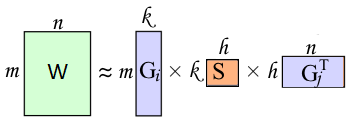
\includegraphics[width=.5\textwidth]{mf2.png}
\caption{Graphical visualization of simultaneous matrix tri-factorization.}
\label{f:mf2}
\end{figure}

In a figure~\ref{f:globokamreza} is shown a neural network with hidden
layers and their relation weight matrices $W_{ij}$ between them. The weight
matrices are collected from neural network and configured in a matrix of
relations $W$ as shown in equation~\ref{eq:1}. A block in the $i$-th
row and $j$-th column ($W_{ij}$) of matrix $W$ represents the relationship
between object type $\xi_i$ and $\xi_j$. In case of a neural network, these
represent neurons at layers $i$ and $j$, respectively. Configuration is set on
diagonal because the neighbour weight matrices share the dimension from shared
hidden layer. The block matrix $W$ is
tri-factorized into block matrix factors $G$ and $S$. A factorization rank
$k_i$ is assigned to $\xi_i$ during inference of the factorized system. Factors
$S_{ij}$ define the relations between layers $\xi_i$ and $\xi_j$, while
factors $G_i$ are specific to layers $\xi_i$ and are used in the
reconstruction of every relation with this layer. In this way, each
weight matrix $W_{ij}$ obtains its own factorization $G_i S_{ij} {G_j}^T$ with
factor $G_i$ ($G_j$) that is shared across relations which involve layers
$\xi_i$ ($\xi_j$). The objective function minimized by penalized matrix
tri-factorization ensures good approximation of the input data and adherence to
must-link and cannot-link constraints~\cite{zitnik2015data}.

\begin{equation} \label{eq:1}
W = 
\begin{bmatrix} 
\begin{smallmatrix}
& &W_{1,2} & & & \\
& & &\ddots & & \\ 
& & & &W_{L-2,L-1} & \\ 
& & & & &W_{L-1,L} 
\end{smallmatrix}
\end{bmatrix} 
\approx 
\begin{bmatrix} 
\begin{smallmatrix}
& &G_1S_{1,2}G_2^T & & & \\ 
& & &\ddots & & \\ 
& & & &G_{L-2}S_{L-2,L-1}G_{L-1}^T & \\ 
& & & & &G_{L-1}S_{L-1,L}G_L^T 
\end{smallmatrix}
\end{bmatrix}
\end{equation}


We can reduce
the number of neurons (parameters) in network as long as the number of 
parameters
in $G_i$ and $G_j$ is less than the number of parameters in $W_{ij}$. If we 
would
like to reduce the number of parameters in $W$ by a fraction of
$p$~\cite{sainath2013low}, we require the equation~\ref{eq:2} to hold.

\begin{equation} \label{eq:2}
 m_1k_1 + k_1h_2 + h_2n_2 + ... + m_{L-1}k_{L-1} + k_{L-1}h_L + h_Ln_L < 
p(m_1n_2 + ... + m_{L-1}n_L)
\end{equation}

\subsection{Approximation of weights in convolutional layers}

With convolutional layers we did not use the same approach. The weights (with 
convolutional networks more regularly called as kernels) in different layers are 
usually independent as they share feature maps with their dimensions dependent 
from each input image. Because of this property we have not found a solution 
based on matrix factorization that considers all connections that exists in all 
layers concurrently. 

In turn we used a non-negative matrix factorization (NMF) method 
for approximation. NMF is
a recent method for finding such a representation. Given a non-negative data 
matrix $W$ (kernel), NMF finds
an approximate factorization $W \approx UV$ into non-negative factors $U$ and 
$V$. The non-negativity
constraints make the representation purely additive (allowing no subtractions), 
in contrast to many
other linear representations~\cite{hoyer2004non}. We used two approaches:
\begin{itemize}
\item In every layer we approximated every kernel separately with NMF. 
\item In every layer we reshaped 
kernels to column vectors and concatenated them into a matrix which we used for 
approximation with NMF (used in pseudocode~\ref{alg:MFBP}).
\end{itemize} Because the kernels in network are not constrained to non-negative 
values, we used a NMF method from Nimfa 
library~\citep{Zitnik2012} which with preprocessing handles negative values in 
input matrix.


\section{Factorization-based brain pruning (MFBP)}
With approximations we determined which weights are better to prune. We pruned
weights which hold followed criteria and were forced to a zero value to be
considered as pruned:

$(abs(originalWeight) - abs(approximatedWeight)) >= threshold$

The pruning procedure is defined in Algorithm~\ref{alg:MFBP}.
The code of pruning modern neural network with simultaneous matrix 
tri-factorization is available online~\cite{code}.

\begin{algorithm}[H]
\label{alg:MFBP}
 \KwData{weight matrices $W$ of learned neural network}
 \KwResult{pruned weight matrices $Wp$}
 \For{every convolutional layer}{
   reshape kernels to column vectors\;
   concatenate kernels into a matrix $W_i$\;
   $A_i$ := approximation of $W_i$ with NMF\;
 }
 \For{every weight matrix $W_i$ in dense connected layers}{
  make relations\;
  add to relations graph $R$;
 }
 apply simultaneous matrix tri-factorization on relations graph $R$\;
 \For{every weight matrix $W$ in relations graph $R$}{
  $A_i$ := approximations of $W_i$\;
 }
 \For{every approximated weight matrix $A$}{
    $Wp_i$ = $W_i$ * (absolute($W_i$) - absolute($A_i$) $<$ threshold)\;
 }
 \caption{Pruning neural network with matrix factorization.}
 
\end{algorithm}



\section{Experimental setup}

We evaluated matrix factorization-based brain pruning on 
MNIST~\cite{lecun-mnisthandwrittendigit-2010} and 
Cifar-10~\cite{krizhevsky2009learning} datasets. 

We used a “modern” neural network, presented in~\cite{github}. There are two
main contributions to a modern neural network. One is changing of activation
function. Instead of sigmoid function it uses a rectifier (Rectified linear 
unit (ReLU) $f(x) = max(0, x)$, where $x$ is the input to a neuron. With
rectifier only the input above zero activates. This
activation function has been argued to be more biologically
plausible~\cite{AISTATS2011_GlorotBB11}. It induces the sparsity in the hidden
neurons and does not face gradient vanishing problem. Deep neural networks
can be trained efficiently using rectifier even without pre-training. 
The other contribution is regularizing the model with
dropout~\cite{srivastava2014dropout}. It addresses
the main problem in deep learning that is overfitting. The purpose of dropout
is to add some noise by “dropping out” a random number of some neuron
activations in a given layer. With every iteration a different random set of
neurons are chosen to drop, therefore it prevents co-adaptation of neurons.
There was also a change of update rule. Instead of a standard stochastic
gradient descent (SGD) backpropagation method we used RMSprop (A mini-batch
version of rpop). The idea behind SGD is to approximate the real update step by
taking the average of the all given mini batches.
RMSprop keeps a running average of its recent gradient magnitudes and divides
the next gradient by this average so that loosely gradient values are
normalized~\cite{lecture}. 

To evaluate our experiments, we implemented algorithm on Python with the help
of Theano~\cite{Bastien-Theano-2012, bergstra+al:2010-scipy}. Theano is a
Python library that is suitable for building an optimized neural network. We
chose it as it gives a comprehensive control over neural network formation
which is suitable for our problem. Another reason we used Theano is because the
implementation of “modern neural net” described above is available 
at~\cite{github}.
Data fusion algorithm which performs simultaneous matrix
tri-factorization is available in a python library
Scikit-fusion~\cite{zitnik2015data}. Algorithm NMF~\cite{Zitnik2012} was used 
for 
pruning in convolutional layers.


\section{Results}
To measure our results with area under ROC 
curve (AUC), we used a machine
learning library Scikit-learn~\cite{scikit-learn}.

\subsection{Results on dense layers}
We trained six neural networks: 
three with two hidden layers and three with four 
hidden layers. Every neural network had 100 iterations available to learn. After 
learning, the simultaneous matrix tri-factorization was performed to prune 
weights. After, 50 iterations of fine-tuning was used to recover the non-pruned 
weight values which have been biased by the pruned weights from before 
pruning. The pruned weights were forced to stay at zero (to keep 
them pruned), so to keep the dimensionality reduction. 
Every type of network had different amount of pruning. 
The reported results are measured  on test set 
shown in figure~\ref{f:results}. 

\begin{figure}[!ht]
\centering
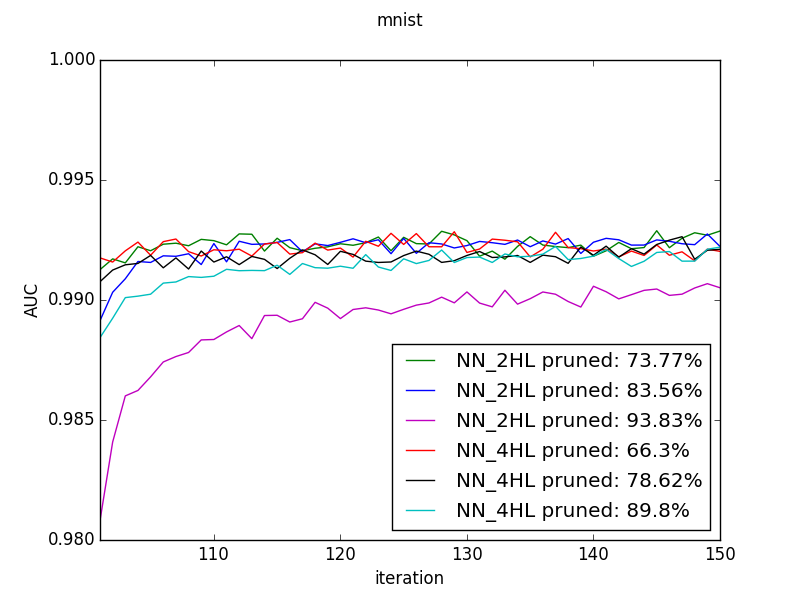
\includegraphics[width=0.8\linewidth]{mnist_new.png}
\captionof{figure}{AUC results of six networks after pruning}
\label{f:results}
\end{figure}

From results we can see 
that the network which had less amount of pruning were able to recover the 
accuracy fast (after few iterations). With higher amount of pruning, 
the non-pruned weights needed more iterations to recover to the accuracy before 
pruning, meanwhile the network with two hidden layers, which was pruned the most 
(for 93,83~\%) was not able to recover as the amount of pruning was too high.
From table~\ref{t:results} we can see that in most cases, the pruning resulted
in higher accuracy than before pruning. 


\begin{table}[!ht]
\centering
\begin{tabular}{l|l|l|p{3cm}|}
\cline{2-4}
 & max AUC score BP & max AUC score AP & a first AUC AP \textgreater= max AUC BP 
\\ \hline
\multicolumn{1}{|l|}{NN\_2HL pruned: 73.77\%} & 0.99272 at 72-iter & 0.99289 at 
145-iter & 0.99275 at 112-iter \\ \hline
\multicolumn{1}{|l|}{NN\_2HL pruned: 83.56\%} & 0.99291 at 88-iter & 0.99275 at 
149-iter & / \\ \hline
\multicolumn{1}{|l|}{NN\_2HL pruned: 93.83\%} & 0.99293 at 83-iter & 0.99068 at 
149-iter & / \\ \hline
\multicolumn{1}{|l|}{NN\_4HL pruned: 66.3\%} & 0.99236 at 97-iter & 0.99284 at 
129-iter & 0.99241 at 104-iter \\ \hline
\multicolumn{1}{|l|}{NN\_4HL pruned: 78.62\%} & 0.99236 at 78-iter & 0.99284 at 
147-iter & 0.99249 at 146-iter \\ \hline
\multicolumn{1}{|l|}{NN\_4HL pruned: 89.8\%} & 0.99201 at 99 iter & 0.99223 at 
137-iter & 0.99208 at 128-iter \\ \hline
\end{tabular}
\caption{AUC results from before pruning (BP) and after pruning (AP).}
\label{t:results}
\end{table}

\subsection{Results on convolutional layers}
We trained a network with three convolutional layers and one dense connected 
layer. We introduced also a CIFAR-10 dataset in this approach. We used two 
previously mentioned approaches of kernel pruning with NMF. We also used 
multiple iterations of pruning, where pruning gets stronger with every 
iteration. Iterations between pruning were reserved for recovering of weights 
that survived. A recovering period was not hard-coded but lasted until there 
were five iterations of recovering where the neurons did not improve for a small 
amount.  

\begin{figure}[!ht]
\centering
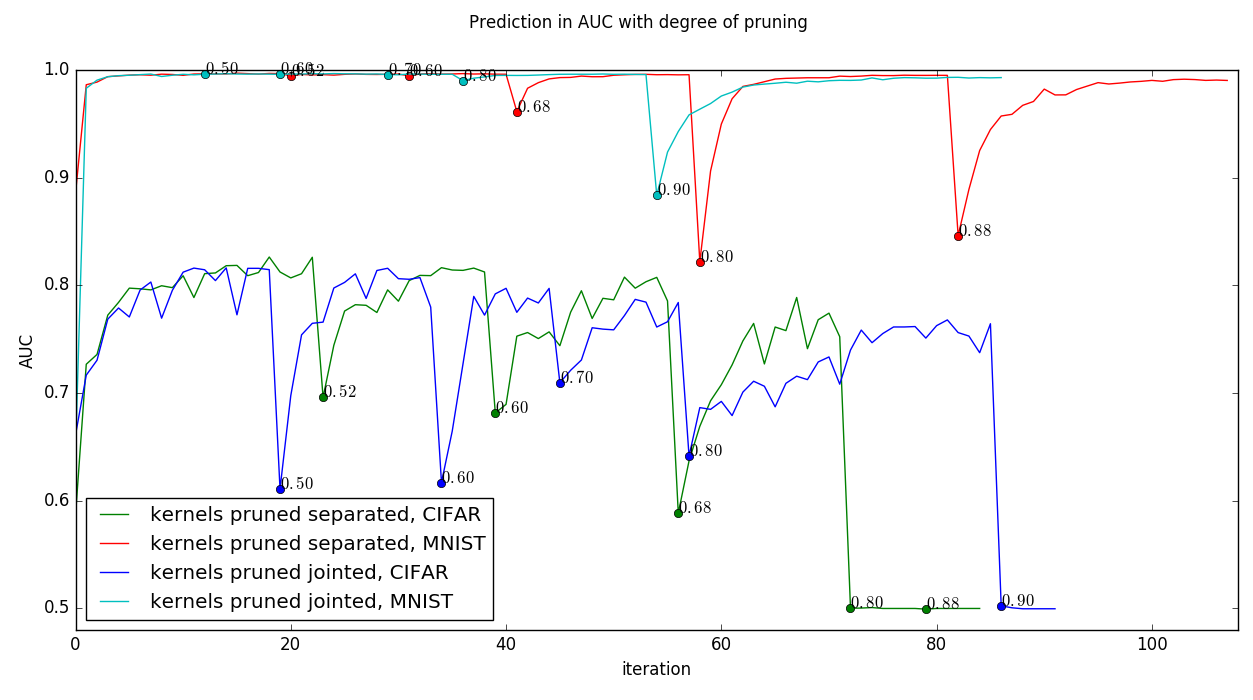
\includegraphics[width=1\linewidth]{convresults.png}
\captionof{figure}{AUC results of two approaches on MNIST and CIFAR dataset.}
\label{f:results_conv}
\end{figure}

\begin{figure}[!ht]
\centering
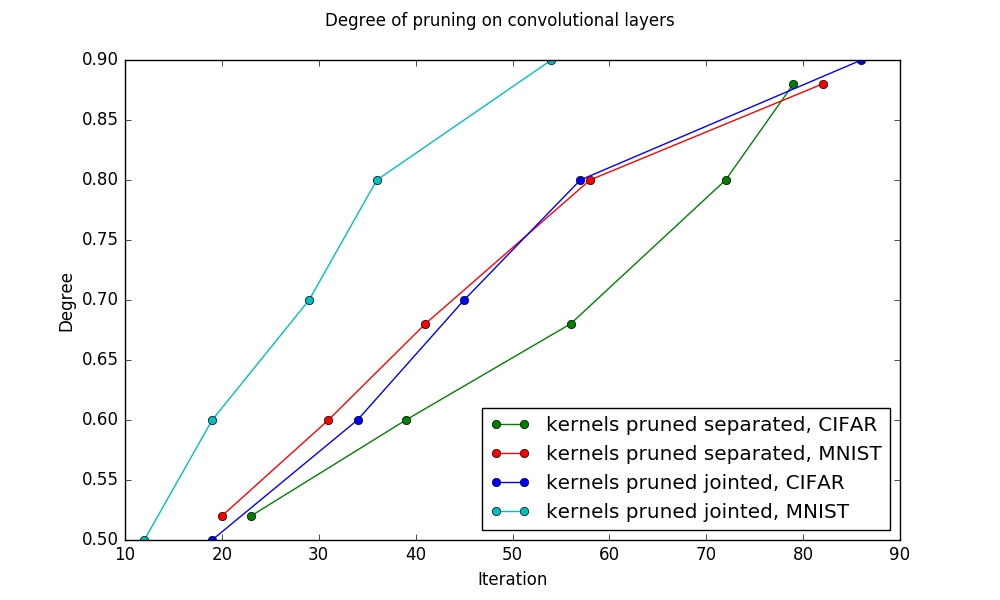
\includegraphics[width=.8\linewidth]{convdegree.png}
\captionof{figure}{Degree of pruning.}
\label{f:degree_conv}
\end{figure}

The results in~\ref{f:results_conv} show four AUC measures, with two approaches 
and two datasets. Pruning occurs at steps where there are coloured dots with a 
number that represents degree of pruning at that step. A 
figure~\ref{f:degree_conv}
separately shows the degree of pruning when pruning occurs.

With results we came to similar conclusions. The network was able to recover 
lost accuracy to some amount. With stronger pruning, the recovery was less 
effective. When we pruned above 80~\% there was a possibility that we lost all 
information that was learned. First, we need to consider that usually, the first 
convolution layer has fewer parameters than the following layers. Secondly it 
directly performs on the input layer and is therefore more sensitive to pruning. 
These reasons may affect the accuracy loss the most. In future, we might 
consider to protect the first layer from strong pruning.


\newpage 
\section{Discussion and conclusion}
In this paper, we have addressed size complexity by applying simultaneous 
matrix tri-factorization to compress network without loss of accuracy. We have 
addressed time complexity 
by applying NMF on kernels to speed up computations. Pruning values in kernels 
has the potential to bridge the gap between pruning and its computational 
advantages. Combined with convolution lowering, it can significantly reduce the 
computational cost~\cite{anwar2015structured}.

We applied matrix factorization on weight matrices and used 
approximated weights to prune the weights which values moved closer to zero for 
the greatest amount. This allowed us to reduce the number of parameters of 
networks between 60-90~\% without sacrificing the accuracy or sacrificing for 
the negligible amount. 

The reduction of the parameters of neural network with 
higher amount of pruning required more iterations of fine-tuning to recover the 
non-pruned 
weights. 

For future work, we will combine pruning on convolutional and dense connected 
layers on a bigger and more serious networks and datasets.
We are planning on conducting experiments on evaluating its effectiveness for 
computational benefits.


%\subsubsection*{Acknowledgments}
%\subsubsection*{References}
\bibliography{literature}
\bibliographystyle{plain}

%\todos

\end{document}








